\documentclass[a4paper, 12pt]{article}
\usepackage{geometry}
\geometry{a4paper,
total={170mm,257mm},left=2cm,right=2cm,
top=2cm,bottom=2cm}

\usepackage{mathtext}
\usepackage{amsmath}
\usepackage[utf8]{inputenc}
\usepackage[english,russian]{babel}
\usepackage{graphicx, float}
\usepackage{tabularx, colortbl}
\usepackage{textcomp}
\usepackage{caption}
\usepackage{wrapfig}
\captionsetup{labelsep=period}

\newcommand{\parag}[1]{\paragraph*{#1:}}
\newcounter{Points}
\setcounter{Points}{1}
\newcommand{\point}{\noindent \arabic{Points}. \addtocounter{Points}{1}}
\newcolumntype{C}{>{\centering\arraybackslash}X}

\author{Калинин Данил, Б01-110}
\date{\today}
\title{Лабораторная работа 1.4.1 \\"Изучение физического маятника"}

\begin{document}
\maketitle

\parag {Цель работы}
исследовать зависимость периода колебаний физического маятника от момента его инерции.
\parag {В работе используются}
физический маятник (однородный стальной стержень), опорная призма, математический маятник, счётчик числа колебаний, линейка, секундомер.

\parag {Теоритическая справка}

\begin{wrapfigure}{l}{7cm}
	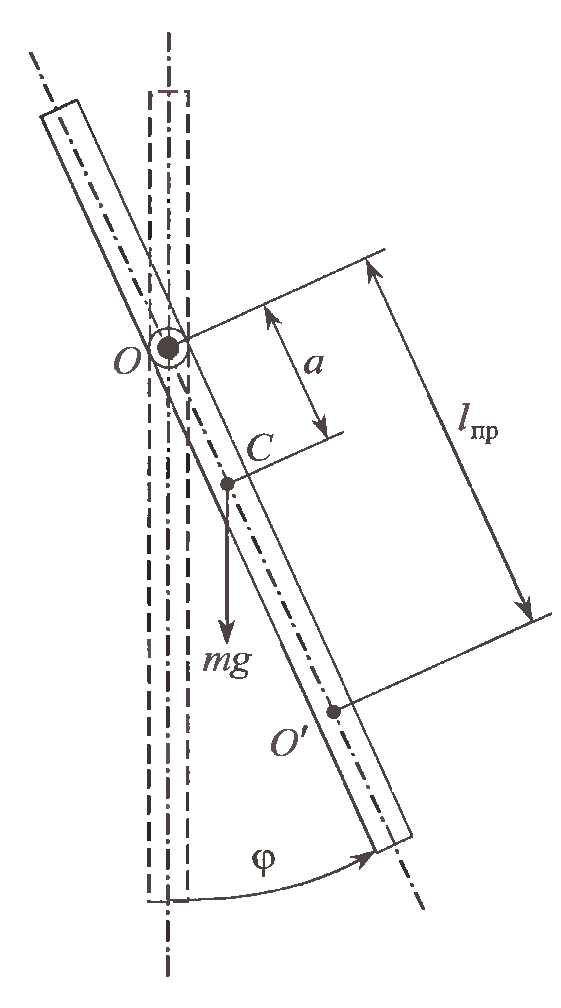
\includegraphics[width=\linewidth]{ustanovka.png}
	\caption{Физический маятник}
    \label{pic:risunok}
\end{wrapfigure}

Физическим маятником называют любое твердое тело, которое под действием силы тяжести может свободно качаться вокруг неподвижной горизонтальной оси. Движение маятника описывается уравнением

\begin{equation}
    I\frac{d^2\varphi}{dt^2}=M,
    \label{eq:osnova}
\end{equation}

\noindent где $ I $ -- момент инерции маятника, $ \varphi $ -- угол отклонения маятника от положения равновесия, $ t $ - время, $ M $ - момент сил, действующих на маятник.

В данной работе в качестве физического маятника (рис.~ \ref{pic:risunok}) используется однородный стальной стержень длиной $ l $. На стержне закрепляется опорная призма, острое ребро которой является осью качания маятника. Призму можно перемещать вдоль стержня, меняя таким образом расстояние $ OC $ от точки опоры маятника до его центра масс. Пусть это расстояние равно $ a $. Тогда по теореме Гюйгенса-Штейнера момент инерции маятника

\begin{equation}
    I=\frac{ml^2}{12}+ma^2,
\end{equation}

\noindent где $ m $ -- масса маятника. Момент силы тяжести, действующий на маятник,

\begin{equation}
    M=-mga\sin\varphi.
\end{equation}

\noindent Если угол $ \varphi $ мал, то $ \sin\varphi\approx\varphi $, так что

\begin{equation}
    M\approx-mga\varphi
\end{equation}

\noindent В исправной установке маятник совершает несколько сот колебаний без заметного затухания. Поэтому моментом силы трения в первом приближении можно пренебречь. Подставляя выражение для $ I $ и $ M $ в \eqref{eq:osnova}, получим уравнение

\begin{equation}
    \ddot{\varphi}+\omega^2\varphi=0,
    \label{eq:phi}
\end{equation}

\noindent где

\begin{equation}
    \omega^2=\frac{ga}{a^2+\frac{l^2}{12}}.
\end{equation}

Тогда период колебаний равен

\begin{equation}
    \label{period}
    T=\frac{2\pi}{\omega}=2\pi\sqrt{\frac{a^2+\frac{l^2}{12}}{ag}}
\end{equation}

Таким образом, период малых колебаний не зависит ни от начальной фазы, ни от амплитуды колебаний. Это утверждение (изохорность) справедливо для колебаний, подчиняющихся уравнению \eqref{eq:phi}. Движение маятника описывается по этой формуле только для малых углов $ \varphi $.

\medskip

Период колебаний математического маятника определяется формулой
\begin{equation}
T'=2\pi\sqrt{\frac{l'}{g}},
\end{equation}
где $ l' $ -- длина математического маятника. Поэтому величину
\begin{equation}
    \label{eq:prived}
    l_\text{пр}=a+\frac{l^2}{12a}
\end{equation}

называют приведённой длиной математического маятника. Поэтому точку $ O' $ (см. рис. \ref{pic:risunok}), отстоящую от точки опоры на расстояние $ l_\text{пр} $, называют центром качания физического маятника. Точка опоры и центр качания маятника обратимы, т.е. при качании маятника вокруг  точки $ O' $ период будет таким же, как и при качании вокруг точки $ O $.


\parag {Ход работы} ~\\
\point Отметим погрешности измерительных приборов:\\

\noindent Секундомер: $ \Delta_c = 0.0001 \text{ с}$ \\
Линейка: $ \Delta_\text{лин} = 0.05 \text{ см}$\\
Штангенциркуль: $ \Delta_\text{штцр} = 0.01 \text{ см}$\\

\noindent \point Измерим параметры стержня

Результаты измерения параметров стержня занесем в таблицу \ref{tabl:start_stats}.

\begin{table}[H]
    \centering
    \begin{tabularx}{\textwidth}
        {|C|C|}
        \hline
        \textbf{Величина} & \textbf{Значение} \\ \hline
        Полная длина стержня & $L = 100 \pm 0.05$ cм. \\ \hline
        Диаметр стержня & $\sigma_{t}^{случ} = 1.62 \pm 0.01$ cм. \\ \hline
        Центр масс стержня & $x_{цм} = 50 \pm 0.05$ cм. \\ \hline
        Центр масс стержня с призмой & $x_{цм} = 51 \pm 0.05$ cм. \\ \hline
        Масса стержня & $m_{ст} = 1.6375$ кг. \\ \hline
        Масса груза & $m_{гр} = 0.3487$ кг. \\ \hline
        Масса призмы & $m_{пр} = 0.0439$ кг. \\ \hline
        Расстояние от центра масс стержня до призмы & $x_{пр} =24 \pm 0.05$ см. \\ \hline

    \end{tabularx}
    \caption{Результаты измерения параметров стержня.}
    \label{tabl:start_stats}
\end{table}

\point Измерим период колебаний маятника без дополнительного груза.
Результат измерения периода колебаний маятника без груза приведен в таблице \ref{tabl:period_for_20_oscillations}.

\begin{table}[H]
    \centering
    \begin{tabularx}{\textwidth}
        {|C|C|C|C|}
        \hline
        \textbf{\textnumero \quad опыта} & \textbf{Кол-во колебаний $N$} & \textbf{Полное время, сек} & \textbf{Расчитанный период, сек} \\ \hline
        \textbf{1 } & 30.62 & 20 & 1.531  \\ \hline
        \textbf{2 } & 30.62 & 20 & 1.531  \\ \hline
        \textbf{3 } & 30.62 & 20 & 1.531  \\ \hline
        \textbf{4 } & 30.63 & 20 & 1.5315 \\ \hline
        \textbf{5 } & 30.63 & 20 & 1.5315 \\ \hline
        \textbf{6 } & 30.63 & 20 & 1.5315 \\ \hline
        \textbf{7 } & 30.63 & 20 & 1.5315 \\ \hline
        \textbf{8 } & 30.63 & 20 & 1.5315 \\ \hline
        \textbf{9 } & 30.62 & 20 & 1.531 \\ \hline
        \textbf{10} & 30.63 & 20 & 1.5315 \\ \hline
    \end{tabularx}
    \caption{Результаты измерения времени 20 колебаний}
    \label{tabl:period_for_20_oscillations}
\end{table}

По полученным данным были расчитанны среднее время $\bar{t}$ 20 полных колебаний, случайная ($\sigma_{t}^{случ}$), систематическая (($\sigma_{t}^{сист}$) и полная ($\sigma_{t}^{полн}$) погрешности измерения времени. Результаты сведены в таблицу \ref{tabl:stats_for_20_oscillations}.

\begin{table}[!h]
    \centering
    \begin{tabularx}{\textwidth}
        {|C|C|}
        \hline
        Среднее время 20 колебаний & $\bar{t} = 30.626$ c. \\ \hline
        Слуйчайная погрешность измерения & $\sigma_{t}^{случ} = 5\cdot10^{-3}$ c. \\ \hline
        Cистематическая погрешность измерения & $\sigma_{t}^{сист} = 1\cdot10^{-3}$ c. \\ \hline
        Полная погрешность измерения & $\sigma_{t}^{сист} = 5.14\cdot10^{-3}$ c. \\ \hline
    \end{tabularx}
    \caption{Результаты измерения времени 20 колебаний.}
    \label{tabl:stats_for_20_oscillations}
\end{table}

\point Рассчитаем $g$.

По данной в описании работы формуле:
\begin{equation}
    g = \frac{4\pi^2(\dfrac{l^2}{12} + a^2)}{T^2a}
\end{equation}

Таким образом получим: $g = 9.83$, $\varepsilon_g = 0.2\%$.

\point Проведем серию измерений, перемещая груз.

\noindent Результаты измерения занесем в таблицу \ref{tabl:moving_weight}. 

\begin{table}[H]
    \centering
    \begin{tabularx}{\textwidth}
        {|C|C|C|C|C|C|}
        \hline
        \textbf{\textnumero \quad Опыта} & \textbf{Координата центра масс стержня, $x_ц$, м.} & \textbf{Расстояние от центра масс стержн до груза $y$, м.} & \textbf{Количество колебаний $n$} & \textbf{Полное время колебаний $t_п$, cек.} & \textbf{Период $T$, сек} \\ \hline
        \textbf{1 } & 0.35 & 0.26 & 4 & 5.83 & 1.457 \\ \hline
        \textbf{2 } & 0.41 & 0.28 & 4 & 5.91 & 1.47 \\ \hline
        \textbf{3 } & 0.37 & 0.27 & 4 & 5.87 & 1.467 \\ \hline
        \textbf{4 } & 0.37 & 0.3  & 4 & 5.97 & 1.492 \\ \hline
        \textbf{5 } & 0.35 & 0.31 & 4 & 6.17 & 1.54 \\ \hline
    \end{tabularx}
    \caption{Результаты измерения периода колебаний при переменном положении груза}
    \label{tabl:moving_weight}
\end{table}

\noindent Расчитаем $J_0$ -- момент инерции маятника.

\begin{equation}
    J_0 = \frac{m_cl^2}{12} + m_ca^2
\end{equation}

\noindent Где $m_c$ -- масса стержня с призмой, $l$ -- длина стержня, $a$ -- расстояние от центра масс стержня до точки подвеса.\\

\noindent Таким образом, получим $J_0 = 0.237 ~ кг \cdot м^2$.\\

\point Рассчитаем значения $g$.
\noindent Из следующей формулы
\begin{equation}
    T = 2\pi\sqrt{\frac{J_0 + m_гy^2}{g^2Mx_ц}}
    \label{eq:period}
\end{equation}

\noindent Выведем следующую формулу для расчета $g$.

\begin{equation}
    g = \frac{4\pi^2(J_0 + m_гy^2)}{T^2Mx_ц}
\end{equation}

\noindent Где $m_г$ -- масса груза, $M$ -- полная масса маятника. 

По формуле расчитаем значения $g$, а также отосительные погрешности (с учетом $g_{ист} = 9.81$) для каждого из измерений, результаты занесем в таблицу \ref{tabl:g}.

\begin{table}[H]
    \centering
    \begin{tabularx}{\textwidth}
        {|C|C|C|}
        \hline
        \textbf{\textnumero \quad Опыта} & \textbf{Рассчитанное значение $g ~ \frac{м}{с^2}$} & \textbf{Ошибка расчета $\varepsilon_g$, \%} \\ \hline
        \textbf{1 } & 9.50 & 3.262 \\ \hline
        \textbf{2 } & 9.85 & 0.44 \\ \hline
        \textbf{3 } & 9.52 & 2.95 \\ \hline
        \textbf{4 } & 8.95 & 9.52 \\ \hline
        \textbf{5 } & 9.37 & 4.68 \\ \hline
    \end{tabularx}
    \caption{Результаты расчетов ускорения свободного падения.}
    \label{tabl:g}
\end{table}

\point Расчитаем случайную погрешность:

\begin{equation}
    \sigma_g^{случ} = \sqrt{\frac{1}{N}\sum_{i=1}^n(\bar{g} - g)^2} 
\end{equation}

Получим $sigm_g = 0.468 ~ \frac{м}{с^2}$. Теперь расчитаем относительную погрешность всей серии измерений:

\begin{equation}
    \varepsilon_g^{серии} =  \frac{\sigma_g^{случ}}{\bar{g}} \cdot 100\%
\end{equation}

Таким образом, $\varepsilon_g^{серии} = 4.97\%$. То есть ускорение свободного падения получено с хорошей точностью.\\

\point Построение графика зависимости периода колебаний от положения груза.

Заметим, что из формулы \ref{eq:period} можно получить следующее уравнение:

\begin{equation}
    T^2x_ц = \frac{4\pi^2}{gM}m_гy^2+\frac{4\pi^2}{gM}J_0.
\end{equation}

\noindent То есть величина $T^2x_ц$ линейно зависит от $y^2$. Иначе говоря:

\begin{equation}
    T^2x_ц = ky^2 + b.
    \label{eq:coef}
\end{equation}
\noindent Где $k = \frac{4\pi^2}{gM}m_г$, а $b = \frac{4\pi^2}{gM}J_0$.

Найдем коэффициенты $k$ и $b$ методом наименьших квадратов:

\begin{equation}
    k=\frac{\langle xy\rangle-\langle x\rangle \langle y\rangle}{\langle x^2\rangle - \langle x\rangle^2} \approx 0.82 \text{ }\frac{\text{с}^2}{\text{м}}
\end{equation}

\begin{equation}
    b=\langle y \rangle -k\langle x \rangle\approx 0.4683 \text{ }\text{см}\cdot\text{с}^2
\end{equation}

где $ x=y^2 $, $ y=x_цT^2 $.

Построим график зависимости $ T^2x_ц$ от $y^2$, пользуясь полученными коэффициентами. На графике отметим экспериментальные точки. График представлен на рисунке \ref{pic:graph}.

\begin{figure}
    \centering
    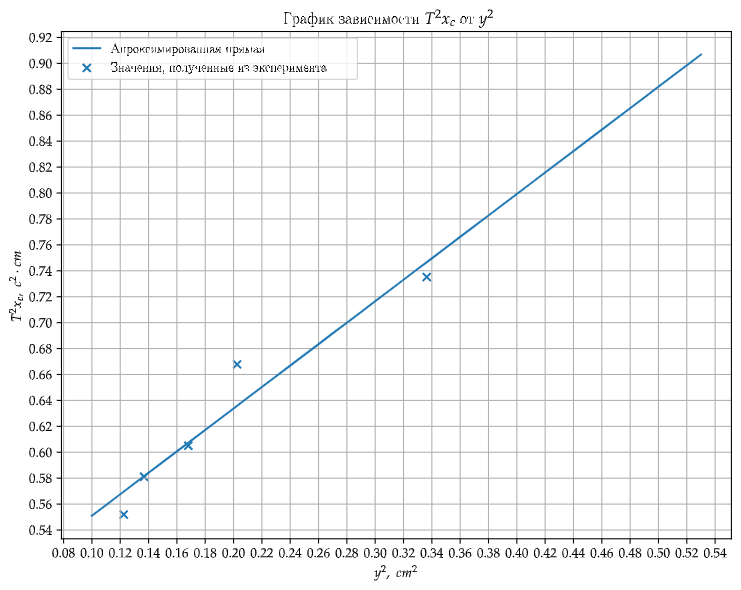
\includegraphics[width=15cm]{plot.png}
	\caption{график зависимости $ T^2x_ц$ от $y^2$}
    \label{pic:graph}
\end{figure}

\point Расчитаем погрешности.

Погрешность расчёта $ y^2 $ найдём по следующей формуле:

\begin{equation}
\sigma_{y^2}=2\Delta y,
\end{equation}
где $ \Delta y = \Delta_{лин} = 0.05$ см.\\

Погрешность вычисления $ x_цT^2 $ можно найти по формуле:

\begin{equation}
\sigma_{x_цT^2} = \sqrt{(\Delta_{лин})^2 + (2\Delta_{сек})^2},
\end{equation}

Случайные погрешности вычисления $ k $ и $ b $ можно найти по следующим формулам:

\begin{equation}
\sigma_k^\text{сл}=\sqrt{\frac{1}{N}\left(\frac{\langle y^2 \rangle - \langle y \rangle^2}{\langle x^2 \rangle - \langle x \rangle^2} - k^2 \right) } \approx 3.34 \cdot 10^{-2} \text{ }\frac{\text{с}^2}{\text{м}},
\end{equation}

\begin{equation}
\sigma_b^\text{сл}= \sigma_k^\text{сл} \sqrt{\langle x^2 \rangle - \langle x \rangle^2} \approx 7.67 \cdot 10^{-3} \text{ }\text{м}\cdot\text{с}^2.
\end{equation}

Относительная погрешность величины $T^2x_ц$:
\begin{equation}
    \varepsilon_{x_цT^2} = \frac{\sigma_{x_цT^2}}{\langle T^2x_ц \rangle} \approx 2.3 \%
\end{equation}

Относительная погрешность величины $y^2$:
\begin{equation}
    \varepsilon_{y^2} = \frac{\sigma_{y^2}}{\langle y^2 \rangle} \approx 0.51 \%
\end{equation}

Систематическая погрешность вычисления коэффициентов определяется следующим соотношением:
\begin{equation}
\sigma^\text{сист}_k = k\sqrt{\left( \varepsilon_{x_цT^2} \right)^2 + \left( \varepsilon_{y^2} \right)^2 } \approx 0.0047 \text{ }\frac{\text{с}^2}{\text{м}},
\end{equation}

\begin{equation}
\sigma^\text{сист}_b = b\sqrt{\left( \varepsilon_{x_цT^2} \right)^2 + \left( \varepsilon_{y^2} \right)^2 } \approx   0.0026 \text{ }\text{м}\cdot\text{с}^2.
\end{equation}

Тогда полную погрешность вычисления коэффициентов подсчитываем по следующей формуле:

\begin{equation}
\sigma_k = \sqrt{\left( \sigma_k^\text{сл} \right)^2 + \left( \sigma_k^\text{сист} \right)^2 } \approx 0.033 \text{ }\frac{\text{с}^2}{\text{м}},
\end{equation}

\begin{equation}
\sigma_b = \sqrt{\left( \sigma_b^\text{сл} \right)^2 + \left( \sigma_b^\text{сист} \right)^2 } \approx 0.0081 \text{ }\text{м}\cdot\text{с}^2.
\end{equation}

Таким образом, получаем:
\begin{itemize}
	\item $ k = (0.82 \pm 0.033) ~\frac{с^2}{м} $,   $ \varepsilon_k = 4.7 \% $
	\item $ b = (0.46 \pm 0.0081) ~ м \cdot с^2 $,    $\varepsilon_b = 1.73 \% $
\end{itemize}


Учитывая формулу \ref{eq:coef} и \ref{eq:period}, вычисляем $g$:

\begin{equation}
    g = \frac{4\pi^2m_г}{Mk} \approx 9.459 ~ \frac{м}{с^2},
\end{equation}
    
\begin{equation}
    \sigma_g = g\cdot\varepsilon_k \approx 0.44 ~ \frac{\text{м}}{\text{с}^2},
\end{equation}

Таким образом получаем:

$g = (9,454 \pm 0,44 ) \frac{\text{м}}{\text{с}^2} $, $ \varepsilon_g=4.654\% $

\parag {Заключение} ~\\
В ходе работы был изучен физический маятник. С хорошей точностью было получено ускорение свободного падения для планеты Земля. Точность можно улучшить, если провести больше экспериментов и увеличить точность измерения расстояния от от груза и точки опоры до центра масс. До сих точность итоговых измерений ограничевается точностью линейки и штангенциркуля. 

\end{document}
